\documentclass{article}
\usepackage[left=2cm,right=2cm,top=2cm,bottom=2cm]{geometry}
\usepackage[utf8]{inputenc}
\usepackage[german]{babel}
\usepackage{amsmath}
\usepackage{dsfont}
\usepackage[export]{adjustbox}
\usepackage{amsthm}
\usepackage{color}
\usepackage{amsfonts}
\usepackage{amssymb}
\usepackage{wasysym}
\usepackage{makeidx}
\usepackage{graphicx}
\usepackage[colorlinks=true,urlcolor=blue,linkcolor=blue]{hyperref}
\usepackage{ziffer}
\usepackage{minted}
\usepackage{xcolor}
\usepackage{framed}
\usepackage{mdframed}
\usepackage{subfiles}
\usemintedstyle{emacs}

\definecolor{purp}{HTML}{9A72AC}
\definecolor{re}{HTML}{FC6255}
\definecolor{gre}{HTML}{83C167}
\definecolor{blu}{HTML}{58C4DD}
\definecolor{shadecolor}{rgb}{0.85,0.85,0.85}
\definecolor{bg}{rgb}{0.95,0.95,0.95}
\setlength{\parindent}{0em} 

\BeforeBeginEnvironment{minted}{\begin{mdframed}[linewidth =2 ,backgroundcolor=bg , linecolor=black, linewidth=0.5]}
\AfterEndEnvironment{minted}{\end{mdframed}}

\newtheorem{defi}{Definition}
\BeforeBeginEnvironment{defi}{\begin{mdframed}[linewidth =2 ,backgroundcolor=bg , linecolor=black, linewidth=0.5]}
\AfterEndEnvironment{defi}{\end{mdframed}}

\newcommand{\bsp}{\textbf{Beispiel}:}
%\newcommand{\task}{\textbf{Aufgabe}:}

\newcommand{\bol}[1]{\textbf{#1}}
\newcommand{\q}[1]{\glqq #1\grqq}
\newcommand{\DODO}[1]{\textbf{\textcolor{red}{DODO:}} #1 \\ \begin{center}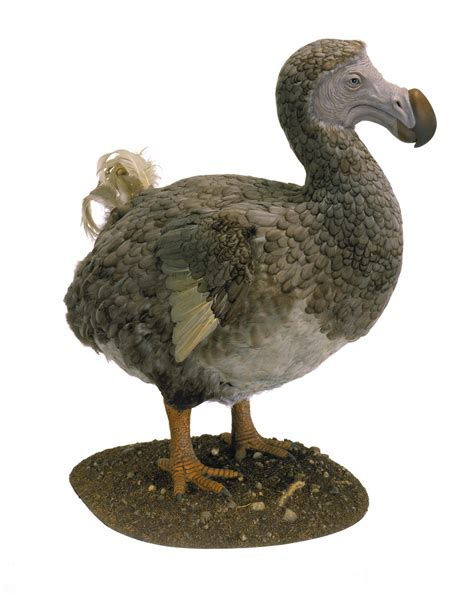
\includegraphics[scale=0.2]{../../media/dodo.jpg} \end{center}}

\newenvironment{task}[1]{
    \begin{shaded*}
    \textbf{Aufgabe #1}:
}{
    \end{shaded*}
}

\begin{document}
In der objektorientierten Programmierung werden häufig \textbf{Entwurfsmuster} verwendet. Sie beschreiben eine Struktur, die in verschiedensten Bereichen Anwendung finden kann. Beim \textbf{Kompositum} handelt es sich um ein Muster, dass Teil-Ganzes-Hierarchien beschreibt. Ein klassisches Beispiel ist die Ordnerstruktur auf einem normalen PC. Ein Ordner kann Dateien, aber auch weitere Ordner enthalten, d.h. auf jeder Ebene kann die Struktur weiter \q{nach unten} wachsen, solange weitere Ordner vorhanden sind. \\
Ein anderes Beispiel sind Bilder aus geometrischen Formen. Jedes Dreieck, Quadrat oder Kreis kann bereits als Bild gesehen werden, zusammengefasst ergeben sie aber wieder ein Bild, das wiederum nur ein Teilbild sein könnte, etc. \\
Ein allgemeines Klassendiagramm der Struktur sieht so aus: 
\begin{center}
    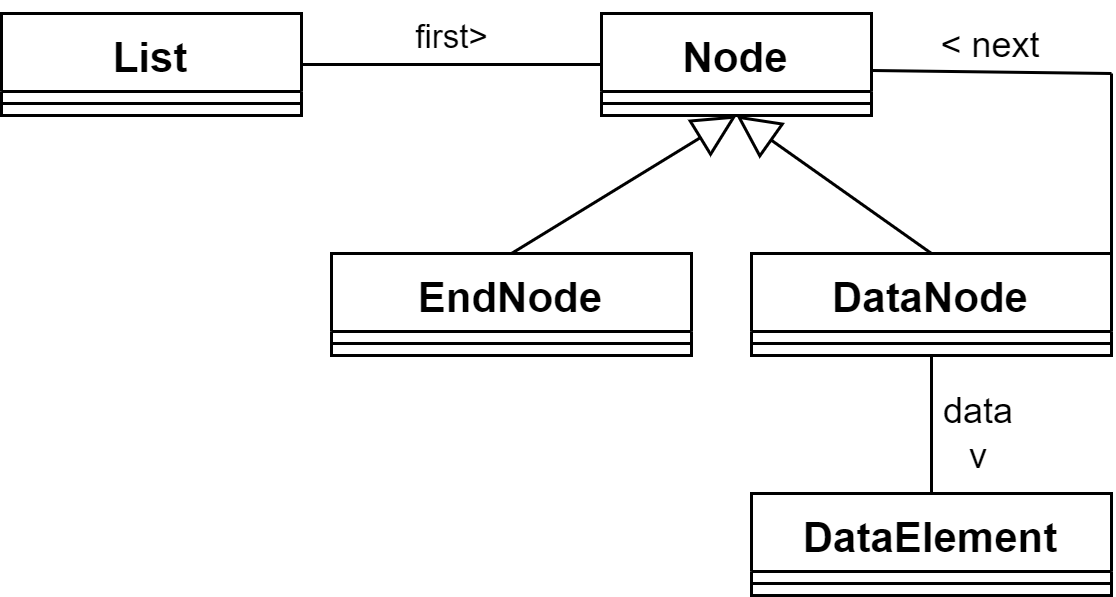
\includegraphics[scale=0.2]{../media/compositum_lists.png}
\end{center}
Die Komponente ist in der Regel eine abstrakte Klasse. In obigem Beispiel wären Dreiecke oder Quadrate Blätter, eine aus zwei Dreiecken zusammengefügte Figur ein Composite, also ein Zusammenschluss aus diesen Objekten. Die Blätter sind die kleinsten Einheiten der Struktur, zu ihnen kann also kein weiteres Objekt hinzugefügt werden. \\
Auf den ersten Blick bringt uns dieses Konzept keine großen Vorteile im Hinblick auf unsere Liste. Wir haben aktuell bereits eine ähnliche Struktur, da jede Teilliste ab einem bestimmten Knoten wieder als Liste gesehen werden könnte. Mit einer kleinen Erweiterung werden wir so aber sogar unsere Null-Referenzprüfungen los: 
\begin{center}
    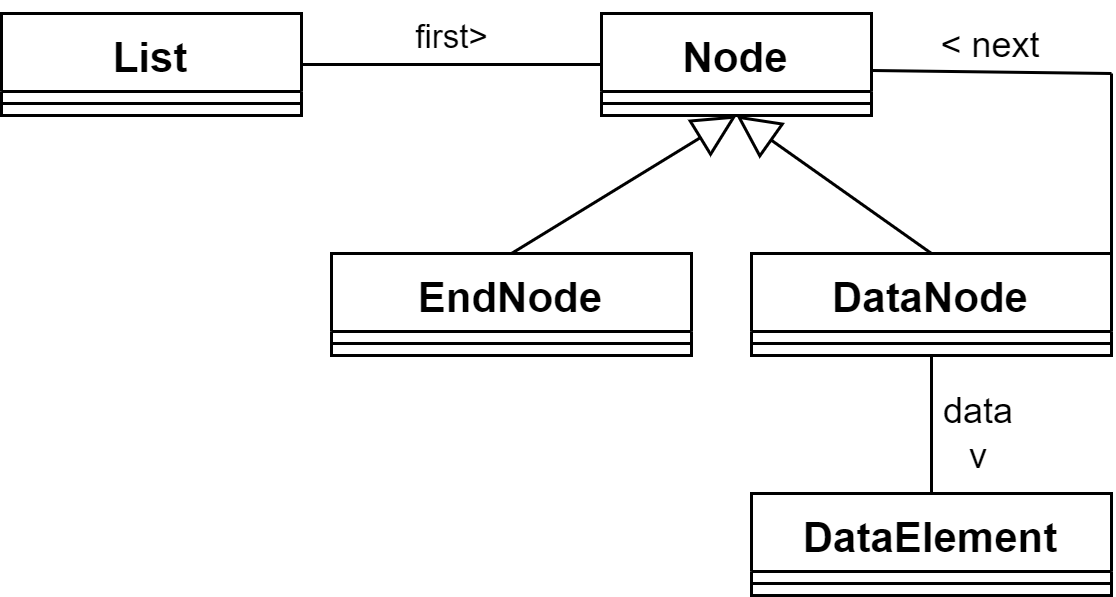
\includegraphics[scale=0.2]{../media/compositum_lists.png}
\end{center}
Unser Blatt, d.h. das Ende unserer Liste wird zu einer eigenen Klasse. Alle Abbruchbedingungen wandern also in diese Klasse, da alle Methoden, die die Liste ganz durchlaufen, zwangsläufig hier ankommen müssen. So kann z.B. das Einfügen eines neuen Knotens ebenfalls durch \q{Durchreichen} der entsprechenden Daten geschehen. Jeder Knoten gibt dabei sich selbst wieder an den Vorgänger als Nachfolger zurück, bis auf den letzten Knoten. Dieser gibt nicht sich selbst, sondern einen neuen Knoten mit sich als Nachfolger zurück und die Liste wurde verlängert. \\
Für die Implementierung beginnen wir wiederum mit dem Grundgerüst. Wir benötigen Klassen für:
\begin{enumerate}
    \item Warteschlange
    \item (abstrakter) Knoten 
    \item Endknoten
    \item Datenknoten
    \item Datenelment
    \item Mensch
\end{enumerate}
\begin{minted}{Java}
    public class MyListComp {
        private Node first;

        public MyListComp() {
            first = new EndNode();
        }
    }
\end{minted}
Der Konstruktor der Warteschlange platziert jetzt keine Null-Referenz mehr, sondern hängt einen Endknoten als Ersten an die Liste an. D.h. die Liste ist jetzt immer mit einem \q{selbst-erstellten} Objekt gefüllt. \\ 
In der Knoten Klasse werden nur die Methodenrümpfe für die tatsächlichen Implementierungen gesetzt (wir könnten diese abstrakte Klasse also auch als Interface implementieren). Für den Moment beschränken wir uns auf die hintenAnfügen() - Methode, die wir im nächsten Schritt implementieren wollen (die Entfernen-Methode ist nicht rekursiv und muss deswegen auch nicht auf den Knoten definiert werden!)
\begin{minted}{Java}
    public abstract class Node {
        public abstract Node push(DataElement data);
    }
\end{minted}
Wer genau hinsieht: Die Methode zum Anfügen eines Knotens hat jetzt einen Rückgabewert! Dies liegt an der bereits oben beschriebenen Vorgehensweise beim Einfügen, dazu später mehr. \\
\begin{minted}{Java}
    public class EndNode extends Node {
        @Override
        public Node push(DataElement data) {
            // TODO
        }
    }
    public class DataNode extends Node {
        private Node next;
        private DataElement data;

        public DataNode(Node node, DataElement data) {
            next = node;
            this.data = data;
        }

        public DataElement getData() {
            return data;
        }

        @Override
        public Node push(DataElement data) {
            // TODO
        }
    }
\end{minted}
Der Endknoten braucht natürlich wieder eine Referenz auf den nächsten Knoten, noch trägt er einen Datensatz, deswegen gibt es in dieser Klasse auch keinerlei Attribute. \\
Im Datenknoten fällt auf, dass die Referenz auf den nächsten Knoten jetzt bereits direkt im Konstruktor als Übergabeparameter gesetzt wird. Diese Implementierung ist wiederum für die rekursiven Methoden nützlich. \\
Es folgt das Datenelement-Interface:
\begin{minted}{Java}
    public interface DataElement {
        public void presentation();
        public boolean isGreater(DataElement data);
        public boolean equals(Object o;)
    }
\end{minted}
Das Interface greift bereits vorweg, da die drei Methoden noch nicht für die Anfügen und Entfernen-Methoden gebraucht werden, sondern nur für die später folgenden Methoden. \\
In der Klasse Mensch sind deswegen dementsprechend bereits alle diese Methoden implementiert. Es ändert sich im Vergleich zur vorherigen Implementierung der verketteten Liste nichts. Auf die getter- und setter-Methoden für die Attribute wurde aus Platzgründen verzichtet.
\begin{minted}{Java}

    public class Human implements DataElement {
    
        private String name;
        private int age; 
    
        public Human(String name, int age){
            this.name = name;
            this.age = age;
        }
    
        @Override
        public void presentation(){
            System.out.println("I am " + name + " and I am " + age + " years old");
        }

        @Override
        public boolean equals(Object o){
            if(this == o) {
                return true;
            }
            if(!(o instanceof Human)){
                return false;
            } 
            Human h = (Human) o;
            if(h.getName() == this.name && h.getAge() == this.age){
                return true;
            } else {
                return false;
            }
        }
    
        @Override
        public boolean isGreater(DataElement data) {
            Human human = null;
            try {
                human = (Human) data;
            } catch (Exception e) {
                System.out.println("The element for the comparison is not a human!");
            }
            if(this.getAge() > human.getAge()) {
                return true;
            }
            return false; 
        }
        
    }    
\end{minted}
Bei der Verwendung der Methoden ist wieder zu beachten, dass die Methode zur Prüfung auf Gleichheit auf Name und Alter zurückgreift, die Methode für die Sortierung allerdings nur auf das Alter. \\
Damit ist unser Gerüst komplett und der Fokus kann auf die Implementierung der hintenAnfügen()-Methode gelegt werden. In der Warteschlangen-Klasse hat sich nur die null-Abfrage verändert. Statt dieser wird nun geprüft, ob der Erste ein Endknoten ist. Falls ja wird ein neuer Datenknoten erzeugt und an die Stelle des alten Ersten gesetzt. \\
\textit{Hinweis:} Der Konstruktor für den Datenknoten erhält die Referenz des \textbf{alten} Ersten, die zu diesem Zeitpunkt noch der Endknoten ist, erst dann wird wieder in die Variable first gespeichert! 
\begin{minted}{Java}
    //class MyListComp
    public void push(DataElement data) {
        first = first.push(data);
    }
\end{minted}
Die Implementierung in der Datenknotenmodellierung ist jetzt sehr schlank: 
\begin{minted}{Java}
    //class DataNode
    public Node push(DataElement data) {
        next = next.push(data);
        return this; 
    }
\end{minted}
Wir müssen hier keine Fallunterscheidung mehr machen, da der betrachtete Knoten sicher nicht das Ende ist, wir müssen lediglich auf dem nächsten Datenknoten wieder die Methode aufrufen. \\
\begin{task}{1}
Überlegen Sie bevor Sie weiterlesen noch einmal selbst, wieso diese Methode einen Knoten zurückgibt und warum der Rückgabewert wieder in der Variable des Nachfolgers gespeichert wird. 
\end{task}
\vspace{2cm}
Anschaulich gesprochen fragt der Datenknoten, ob sein Nachfolger noch derselbe bleibt, denn das Ergebnis des Methodenaufrufs wird im Nachfolger gespeichert. Anschließend gibt er sich selbst zurück, damit sein Vorgänger den Knoten wieder in der entsprechenden Referenz speichern kann. Es soll sich bei keinem Knoten außer dem letzten die Referenz verändern! \\
Kommen wir beim Endknoten an, so soll dieser Endknoten nicht mehr sich selbst zurückgeben, sondern einen neuen Datenknoten. Das bedeutet, der vormals letzte Knoten erhält als Referenz den neuen Knoten zurück! 
\begin{minted}{Java}
    //class EndNode
    public Node push(DataElement data) {
        return new DataNode(this, data);
    }
\end{minted}
Veranschaulicht in einem \href{https://youtu.be/1YPStkwFbKI}{Video}:
\begin{task}{2}
    Implementieren Sie die vorneEntfernen() und auflisten()- Methode selbstständig, bevor Sie weiterlesen. 
\end{task}
\vspace{3cm}
Um die Grundfunktionalität wiederherzustellen sind die in der vorherigen Aufgabe erwähnten Methoden nötig:
\begin{minted}{Java}
    //class MyListComp
    public DataElement pop() {
        DataElement toReturn = first.getData();
        first = first.getNext();
        return toReturn;
    }
    public void printList() {
        first.printList();
    }
\end{minted}
Es bietet sich für alle rekursiven Methoden an, einen Eintrag in der abstrakten Klasse Knoten zu hinterlassen, um die Implementierung zu erwzingen (auch wenn in der Endknoten-Kasse gegebenenfalls nichts passiert, die Methode muss auch auf dieser Art von Knoten aufrufbar sein, um den Abbruch einzuleiten!).
\begin{minted}{Java}
    //class Node
    public abstract void printList();

    //class DataNode
    public void printList() {
        data.presentation();
        next.printList(); 
    }

    //class EndNode 
    public void printList() {
        System.out.println("This is the end!");
        return;    
    }
\end{minted}

Es folgt der bereits altbekannte Aufgabenblock, alle rekursiven Methoden sollen möglichst die Struktur des Kompositums ausnutzen und innerhalb der Knotenimplementierungen auf instanceof-Verwendungen verzichten. (In der Warteschlangen-Klasse ist dies i.d.R. nicht vermeidbar). Die Lösungen für die ersten sieben Aufgaben finden sich kommentiert auf den folgenden Seiten. Der reine Quellcode (auch für die Experten-Aufgaben 8 und 9) ist in einem seperaten pdf zusammengestellt, sowie auf mebis und github verfügbar. \\ 

\begin{task}{3} 
    Schreiben  Sie eine Methode länge() (length()), die die aktuelle Länge der Warteschlange bestimmt und zurückgibt.   
\end{task}

\begin{task}{4}
    Schreiben Sie eine Methode itemAnPosition(int position) (itemAtPosition(int position)), die eine Referenz zum Listenelement an der angegebenen Position zurückgibt. Beachten Sie Grenz- bzw. Spezialfälle!
\end{task}
    
\begin{task}{5}
    Schreiben Sie eine Methode sucheInSchlange(Datenelement d) (searchItemInQueue(DataElement d)), die die Position des Datenelements in der Schlange zurückgibt. \\
\end{task}
    
\begin{task}{6}
    Schreiben Sie eine Methode enthält(DataElement d) (contains(DataElement d)), die wahr zurückgibt, wenn das Datenelement in der Schlange ist, anderfalls falsch.
\end{task}
\begin{task}{7}
    Schreiben Sie eine Methode entferneAnPosition(int position) (removeAtPosition(int position)), die das Datenelement an der gegebenen Stelle entfernt.\\
    Schreiben Sie zwei Versionen dieser Methode, eine, die das Datenelement nur entfernt und eine, die eine Referenz zu diesem Element zurückgibt.
\end{task}

\begin{task}{8}
Schreiben Sie eine Methode Knoten entferneElement(Datenelement zuEntfernen) (Node removeElement(DataElement toRemove)) und adaptieren Sie das Vorgehen der hintenAnfügen()-Methode, um die Struktur des \q{Durchreichens} zu verwenden.
\end{task}

\begin{task}{9 - für Experten}
    Schreiben Sie eine Methode zusammenfügen(MeineListeComp zweiteWarteschlange) (concatenate(MyListComp secondQueue)), die eine zusammengefügte Liste zurückgibt. 
\end{task}
    
\begin{task}{10 - für Experten}
    Schreiben Sie eine Methode fügeSortiertHinzu(Datenelement d) (appendSorted(DataElement d)), die die Warteschlange nicht von hinten auffüllt, sondern die Menschen an einer bestimmten Stelle einsortiert. \\
    \end{task}
    
\begin{task}{11 - frei}
    Überlegen Sie sich eigene, sinnvolle weitere Methoden für die Warteschlangen-Implementierung.
\end{task}

\end{document}